% SOURCE: edit-harness/results/frame_a/cells/cell_*_real_MIX_{A,B,C}_*.json
% !TEX encoding = UTF-8 Unicode
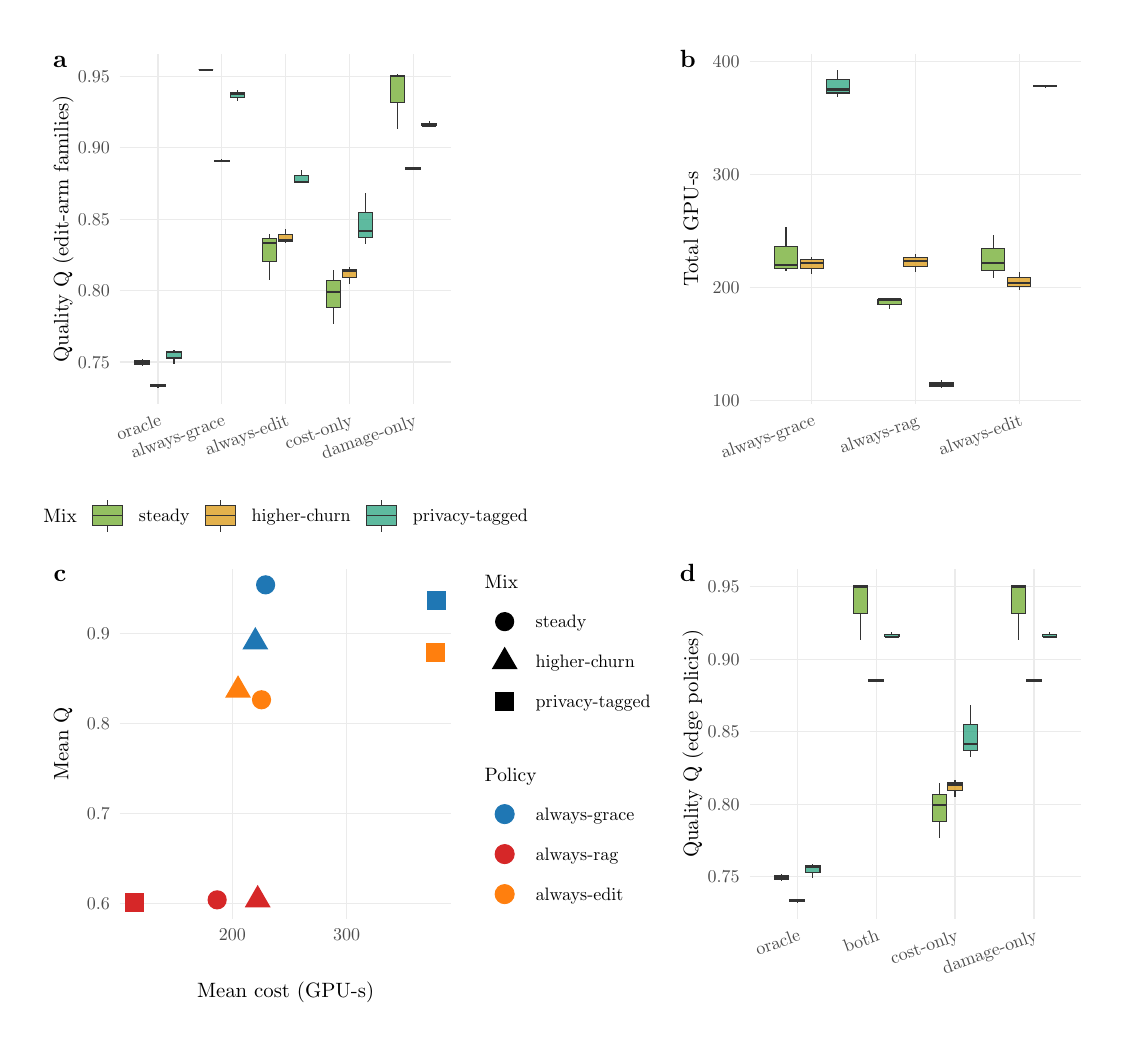
\begin{tikzpicture}[x=1pt,y=1pt]
\definecolor{fillColor}{RGB}{255,255,255}
\path[use as bounding box,fill=fillColor,fill opacity=0.00] (0,0) rectangle (390.26,361.35);
\begin{scope}
\path[clip] (  0.00,  0.00) rectangle (390.26,361.35);
\definecolor{drawColor}{RGB}{255,255,255}
\definecolor{fillColor}{RGB}{255,255,255}

\path[draw=drawColor,line width= 0.6pt,line join=round,line cap=round,fill=fillColor] (  0.00,  0.00) rectangle (390.26,361.35);
\end{scope}
\begin{scope}
\path[clip] (  5.50,169.76) rectangle (233.12,355.85);
\definecolor{fillColor}{RGB}{255,255,255}

\path[fill=fillColor] (  5.50,169.76) rectangle (233.12,355.85);
\end{scope}
\begin{scope}
\path[clip] (233.12,169.76) rectangle (384.76,355.85);
\definecolor{fillColor}{RGB}{255,255,255}

\path[fill=fillColor] (233.12,169.76) rectangle (384.76,355.85);
\end{scope}
\begin{scope}
\path[clip] (  5.50,  5.50) rectangle (233.12,169.76);
\definecolor{fillColor}{RGB}{255,255,255}

\path[fill=fillColor] (  5.50,  5.50) rectangle (233.12,169.76);
\end{scope}
\begin{scope}
\path[clip] (233.12,  5.50) rectangle (384.76,169.76);
\definecolor{fillColor}{RGB}{255,255,255}

\path[fill=fillColor] (233.12,  5.50) rectangle (384.76,169.76);
\end{scope}
\begin{scope}
\path[clip] ( 33.28,225.49) rectangle (153.13,351.85);
\definecolor{drawColor}{gray}{0.92}

\path[draw=drawColor,line width= 0.4pt,line join=round] ( 33.28,240.54) --
	(153.13,240.54);

\path[draw=drawColor,line width= 0.4pt,line join=round] ( 33.28,266.36) --
	(153.13,266.36);

\path[draw=drawColor,line width= 0.4pt,line join=round] ( 33.28,292.19) --
	(153.13,292.19);

\path[draw=drawColor,line width= 0.4pt,line join=round] ( 33.28,318.01) --
	(153.13,318.01);

\path[draw=drawColor,line width= 0.4pt,line join=round] ( 33.28,343.83) --
	(153.13,343.83);

\path[draw=drawColor,line width= 0.4pt,line join=round] ( 47.11,225.49) --
	( 47.11,351.85);

\path[draw=drawColor,line width= 0.4pt,line join=round] ( 70.16,225.49) --
	( 70.16,351.85);

\path[draw=drawColor,line width= 0.4pt,line join=round] ( 93.21,225.49) --
	( 93.21,351.85);

\path[draw=drawColor,line width= 0.4pt,line join=round] (116.25,225.49) --
	(116.25,351.85);

\path[draw=drawColor,line width= 0.4pt,line join=round] (139.30,225.49) --
	(139.30,351.85);
\definecolor{drawColor}{gray}{0.20}

\path[draw=drawColor,line width= 0.4pt,line join=round] ( 41.34,240.95) -- ( 41.34,241.57);

\path[draw=drawColor,line width= 0.4pt,line join=round] ( 41.34,239.71) -- ( 41.34,239.09);
\definecolor{fillColor}{RGB}{102,166,31}

\path[draw=drawColor,line width= 0.4pt,fill=fillColor,fill opacity=0.70] ( 38.75,240.95) --
	( 38.75,239.71) --
	( 43.94,239.71) --
	( 43.94,240.95) --
	( 38.75,240.95) --
	cycle;

\path[draw=drawColor,line width= 0.8pt] ( 38.75,240.33) -- ( 43.94,240.33);

\path[draw=drawColor,line width= 0.4pt,line join=round] ( 47.11,232.27) -- ( 47.11,232.48);

\path[draw=drawColor,line width= 0.4pt,line join=round] ( 47.11,231.65) -- ( 47.11,231.24);
\definecolor{fillColor}{RGB}{216,144,0}

\path[draw=drawColor,line width= 0.4pt,fill=fillColor,fill opacity=0.70] ( 44.51,232.27) --
	( 44.51,231.65) --
	( 49.70,231.65) --
	( 49.70,232.27) --
	( 44.51,232.27) --
	cycle;

\path[draw=drawColor,line width= 0.8pt] ( 44.51,232.06) -- ( 49.70,232.06);

\path[draw=drawColor,line width= 0.4pt,line join=round] ( 52.87,244.47) -- ( 52.87,244.88);

\path[draw=drawColor,line width= 0.4pt,line join=round] ( 52.87,241.99) -- ( 52.87,239.92);
\definecolor{fillColor}{RGB}{27,158,119}

\path[draw=drawColor,line width= 0.4pt,fill=fillColor,fill opacity=0.70] ( 50.28,244.47) --
	( 50.28,241.99) --
	( 55.46,241.99) --
	( 55.46,244.47) --
	( 50.28,244.47) --
	cycle;

\path[draw=drawColor,line width= 0.8pt] ( 50.28,244.05) -- ( 55.46,244.05);

\path[draw=drawColor,line width= 0.4pt,line join=round] ( 64.39,346.11) -- ( 64.39,346.11);

\path[draw=drawColor,line width= 0.4pt,line join=round] ( 64.39,346.11) -- ( 64.39,346.11);
\definecolor{fillColor}{RGB}{102,166,31}

\path[draw=drawColor,line width= 0.4pt,fill=fillColor,fill opacity=0.70] ( 61.80,346.11) --
	( 61.80,346.11) --
	( 66.99,346.11) --
	( 66.99,346.11) --
	( 61.80,346.11) --
	cycle;

\path[draw=drawColor,line width= 0.8pt] ( 61.80,346.11) -- ( 66.99,346.11);

\path[draw=drawColor,line width= 0.4pt,line join=round] ( 70.16,313.46) -- ( 70.16,313.87);

\path[draw=drawColor,line width= 0.4pt,line join=round] ( 70.16,313.05) -- ( 70.16,313.05);
\definecolor{fillColor}{RGB}{216,144,0}

\path[draw=drawColor,line width= 0.4pt,fill=fillColor,fill opacity=0.70] ( 67.56,313.46) --
	( 67.56,313.05) --
	( 72.75,313.05) --
	( 72.75,313.46) --
	( 67.56,313.46) --
	cycle;

\path[draw=drawColor,line width= 0.8pt] ( 67.56,313.05) -- ( 72.75,313.05);

\path[draw=drawColor,line width= 0.4pt,line join=round] ( 75.92,338.05) -- ( 75.92,338.67);

\path[draw=drawColor,line width= 0.4pt,line join=round] ( 75.92,336.19) -- ( 75.92,334.95);
\definecolor{fillColor}{RGB}{27,158,119}

\path[draw=drawColor,line width= 0.4pt,fill=fillColor,fill opacity=0.70] ( 73.32,338.05) --
	( 73.32,336.19) --
	( 78.51,336.19) --
	( 78.51,338.05) --
	( 73.32,338.05) --
	cycle;

\path[draw=drawColor,line width= 0.8pt] ( 73.32,337.43) -- ( 78.51,337.43);

\path[draw=drawColor,line width= 0.4pt,line join=round] ( 87.44,285.08) -- ( 87.44,286.73);

\path[draw=drawColor,line width= 0.4pt,line join=round] ( 87.44,276.77) -- ( 87.44,270.11);
\definecolor{fillColor}{RGB}{102,166,31}

\path[draw=drawColor,line width= 0.4pt,fill=fillColor,fill opacity=0.70] ( 84.85,285.08) --
	( 84.85,276.77) --
	( 90.04,276.77) --
	( 90.04,285.08) --
	( 84.85,285.08) --
	cycle;

\path[draw=drawColor,line width= 0.8pt] ( 84.85,283.42) -- ( 90.04,283.42);

\path[draw=drawColor,line width= 0.4pt,line join=round] ( 93.21,286.57) -- ( 93.21,288.65);

\path[draw=drawColor,line width= 0.4pt,line join=round] ( 93.21,284.06) -- ( 93.21,283.61);
\definecolor{fillColor}{RGB}{216,144,0}

\path[draw=drawColor,line width= 0.4pt,fill=fillColor,fill opacity=0.70] ( 90.61,286.57) --
	( 90.61,284.06) --
	( 95.80,284.06) --
	( 95.80,286.57) --
	( 90.61,286.57) --
	cycle;

\path[draw=drawColor,line width= 0.8pt] ( 90.61,284.50) -- ( 95.80,284.50);

\path[draw=drawColor,line width= 0.4pt,line join=round] ( 98.97,307.90) -- ( 98.97,310.08);

\path[draw=drawColor,line width= 0.4pt,line join=round] ( 98.97,305.64) -- ( 98.97,305.57);
\definecolor{fillColor}{RGB}{27,158,119}

\path[draw=drawColor,line width= 0.4pt,fill=fillColor,fill opacity=0.70] ( 96.37,307.90) --
	( 96.37,305.64) --
	(101.56,305.64) --
	(101.56,307.90) --
	( 96.37,307.90) --
	cycle;

\path[draw=drawColor,line width= 0.8pt] ( 96.37,305.72) -- (101.56,305.72);

\path[draw=drawColor,line width= 0.4pt,line join=round] (110.49,269.91) -- (110.49,273.90);

\path[draw=drawColor,line width= 0.4pt,line join=round] (110.49,260.17) -- (110.49,254.40);
\definecolor{fillColor}{RGB}{102,166,31}

\path[draw=drawColor,line width= 0.4pt,fill=fillColor,fill opacity=0.70] (107.90,269.91) --
	(107.90,260.17) --
	(113.09,260.17) --
	(113.09,269.91) --
	(107.90,269.91) --
	cycle;

\path[draw=drawColor,line width= 0.8pt] (107.90,265.93) -- (113.09,265.93);

\path[draw=drawColor,line width= 0.4pt,line join=round] (116.25,274.09) -- (116.25,274.84);

\path[draw=drawColor,line width= 0.4pt,line join=round] (116.25,271.07) -- (116.25,268.80);
\definecolor{fillColor}{RGB}{216,144,0}

\path[draw=drawColor,line width= 0.4pt,fill=fillColor,fill opacity=0.70] (113.66,274.09) --
	(113.66,271.07) --
	(118.85,271.07) --
	(118.85,274.09) --
	(113.66,274.09) --
	cycle;

\path[draw=drawColor,line width= 0.8pt] (113.66,273.34) -- (118.85,273.34);

\path[draw=drawColor,line width= 0.4pt,line join=round] (122.02,294.72) -- (122.02,301.65);

\path[draw=drawColor,line width= 0.4pt,line join=round] (122.02,285.52) -- (122.02,283.25);
\definecolor{fillColor}{RGB}{27,158,119}

\path[draw=drawColor,line width= 0.4pt,fill=fillColor,fill opacity=0.70] (119.42,294.72) --
	(119.42,285.52) --
	(124.61,285.52) --
	(124.61,294.72) --
	(119.42,294.72) --
	cycle;

\path[draw=drawColor,line width= 0.8pt] (119.42,287.78) -- (124.61,287.78);

\path[draw=drawColor,line width= 0.4pt,line join=round] (133.54,344.22) -- (133.54,344.51);

\path[draw=drawColor,line width= 0.4pt,line join=round] (133.54,334.41) -- (133.54,324.91);
\definecolor{fillColor}{RGB}{102,166,31}

\path[draw=drawColor,line width= 0.4pt,fill=fillColor,fill opacity=0.70] (130.95,344.22) --
	(130.95,334.41) --
	(136.14,334.41) --
	(136.14,344.22) --
	(130.95,344.22) --
	cycle;

\path[draw=drawColor,line width= 0.8pt] (130.95,343.92) -- (136.14,343.92);

\path[draw=drawColor,line width= 0.4pt,line join=round] (139.30,310.64) -- (139.30,310.99);

\path[draw=drawColor,line width= 0.4pt,line join=round] (139.30,310.12) -- (139.30,309.97);
\definecolor{fillColor}{RGB}{216,144,0}

\path[draw=drawColor,line width= 0.4pt,fill=fillColor,fill opacity=0.70] (136.71,310.64) --
	(136.71,310.12) --
	(141.90,310.12) --
	(141.90,310.64) --
	(136.71,310.64) --
	cycle;

\path[draw=drawColor,line width= 0.8pt] (136.71,310.28) -- (141.90,310.28);

\path[draw=drawColor,line width= 0.4pt,line join=round] (145.07,326.78) -- (145.07,327.59);

\path[draw=drawColor,line width= 0.4pt,line join=round] (145.07,325.96) -- (145.07,325.93);
\definecolor{fillColor}{RGB}{27,158,119}

\path[draw=drawColor,line width= 0.4pt,fill=fillColor,fill opacity=0.70] (142.47,326.78) --
	(142.47,325.96) --
	(147.66,325.96) --
	(147.66,326.78) --
	(142.47,326.78) --
	cycle;

\path[draw=drawColor,line width= 0.8pt] (142.47,325.98) -- (147.66,325.98);
\end{scope}
\begin{scope}
\path[clip] (  0.00,  0.00) rectangle (390.26,361.35);
\definecolor{drawColor}{gray}{0.30}

\node[text=drawColor,anchor=base east,inner sep=0pt, outer sep=0pt, scale=  0.65] at ( 29.68,238.30) {0.75};

\node[text=drawColor,anchor=base east,inner sep=0pt, outer sep=0pt, scale=  0.65] at ( 29.68,264.13) {0.80};

\node[text=drawColor,anchor=base east,inner sep=0pt, outer sep=0pt, scale=  0.65] at ( 29.68,289.95) {0.85};

\node[text=drawColor,anchor=base east,inner sep=0pt, outer sep=0pt, scale=  0.65] at ( 29.68,315.77) {0.90};

\node[text=drawColor,anchor=base east,inner sep=0pt, outer sep=0pt, scale=  0.65] at ( 29.68,341.60) {0.95};
\end{scope}
\begin{scope}
\path[clip] (  0.00,  0.00) rectangle (390.26,361.35);
\definecolor{drawColor}{gray}{0.30}

\node[text=drawColor,rotate= 20.00,anchor=base east,inner sep=0pt, outer sep=0pt, scale=  0.65] at ( 48.64,217.69) {oracle};

\node[text=drawColor,rotate= 20.00,anchor=base east,inner sep=0pt, outer sep=0pt, scale=  0.65] at ( 71.69,217.69) {always-grace};

\node[text=drawColor,rotate= 20.00,anchor=base east,inner sep=0pt, outer sep=0pt, scale=  0.65] at ( 94.74,217.69) {always-edit};

\node[text=drawColor,rotate= 20.00,anchor=base east,inner sep=0pt, outer sep=0pt, scale=  0.65] at (117.79,217.69) {cost-only};

\node[text=drawColor,rotate= 20.00,anchor=base east,inner sep=0pt, outer sep=0pt, scale=  0.65] at (140.84,217.69) {damage-only};
\end{scope}
\begin{scope}
\path[clip] (  0.00,  0.00) rectangle (390.26,361.35);
\definecolor{drawColor}{RGB}{0,0,0}

\node[text=drawColor,rotate= 90.00,anchor=base,inner sep=0pt, outer sep=0pt, scale=  0.75] at ( 14.67,288.67) {Quality Q (edit-arm families)};
\end{scope}
\begin{scope}
\path[clip] (  0.00,  0.00) rectangle (390.26,361.35);
\definecolor{drawColor}{RGB}{0,0,0}

\node[text=drawColor,anchor=base west,inner sep=0pt, outer sep=0pt, scale=  0.70] at (  5.71,182.58) {Mix};
\end{scope}
\begin{scope}
\path[clip] (  0.00,  0.00) rectangle (390.26,361.35);
\definecolor{drawColor}{gray}{0.20}

\path[draw=drawColor,line width= 0.4pt] ( 28.99,179.21) --
	( 28.99,181.37);

\path[draw=drawColor,line width= 0.4pt] ( 28.99,188.60) --
	( 28.99,190.77);
\definecolor{fillColor}{RGB}{102,166,31}

\path[draw=drawColor,line width= 0.4pt,fill=fillColor,fill opacity=0.70] ( 23.57,181.37) rectangle ( 34.41,188.60);

\path[draw=drawColor,line width= 0.4pt] ( 23.57,184.99) --
	( 34.41,184.99);

\path[draw=drawColor,line width= 0.4pt] ( 28.99,179.21) --
	( 28.99,179.21);

\path[draw=drawColor,line width= 0.4pt] ( 28.99,190.77) --
	( 28.99,190.77);
\end{scope}
\begin{scope}
\path[clip] (  0.00,  0.00) rectangle (390.26,361.35);
\definecolor{drawColor}{gray}{0.20}

\path[draw=drawColor,line width= 0.4pt] ( 69.71,179.21) --
	( 69.71,181.37);

\path[draw=drawColor,line width= 0.4pt] ( 69.71,188.60) --
	( 69.71,190.77);
\definecolor{fillColor}{RGB}{216,144,0}

\path[draw=drawColor,line width= 0.4pt,fill=fillColor,fill opacity=0.70] ( 64.29,181.37) rectangle ( 75.13,188.60);

\path[draw=drawColor,line width= 0.4pt] ( 64.29,184.99) --
	( 75.13,184.99);

\path[draw=drawColor,line width= 0.4pt] ( 69.71,179.21) --
	( 69.71,179.21);

\path[draw=drawColor,line width= 0.4pt] ( 69.71,190.77) --
	( 69.71,190.77);
\end{scope}
\begin{scope}
\path[clip] (  0.00,  0.00) rectangle (390.26,361.35);
\definecolor{drawColor}{gray}{0.20}

\path[draw=drawColor,line width= 0.4pt] (127.94,179.21) --
	(127.94,181.37);

\path[draw=drawColor,line width= 0.4pt] (127.94,188.60) --
	(127.94,190.77);
\definecolor{fillColor}{RGB}{27,158,119}

\path[draw=drawColor,line width= 0.4pt,fill=fillColor,fill opacity=0.70] (122.52,181.37) rectangle (133.36,188.60);

\path[draw=drawColor,line width= 0.4pt] (122.52,184.99) --
	(133.36,184.99);

\path[draw=drawColor,line width= 0.4pt] (127.94,179.21) --
	(127.94,179.21);

\path[draw=drawColor,line width= 0.4pt] (127.94,190.77) --
	(127.94,190.77);
\end{scope}
\begin{scope}
\path[clip] (  0.00,  0.00) rectangle (390.26,361.35);
\definecolor{drawColor}{RGB}{0,0,0}

\node[text=drawColor,anchor=base west,inner sep=0pt, outer sep=0pt, scale=  0.65] at ( 40.21,182.75) {steady};
\end{scope}
\begin{scope}
\path[clip] (  0.00,  0.00) rectangle (390.26,361.35);
\definecolor{drawColor}{RGB}{0,0,0}

\node[text=drawColor,anchor=base west,inner sep=0pt, outer sep=0pt, scale=  0.65] at ( 80.94,182.75) {higher-churn};
\end{scope}
\begin{scope}
\path[clip] (  0.00,  0.00) rectangle (390.26,361.35);
\definecolor{drawColor}{RGB}{0,0,0}

\node[text=drawColor,anchor=base west,inner sep=0pt, outer sep=0pt, scale=  0.65] at (139.17,182.75) {privacy-tagged};
\end{scope}
\begin{scope}
\path[clip] (  0.00,  0.00) rectangle (390.26,361.35);
\definecolor{drawColor}{RGB}{0,0,0}

\node[text=drawColor,anchor=base,inner sep=0pt, outer sep=0pt, scale=  0.90] at ( 11.70,346.96) {\bfseries a};
\end{scope}
\begin{scope}
\path[clip] (260.90,225.49) rectangle (380.76,351.85);
\definecolor{drawColor}{gray}{0.92}

\path[draw=drawColor,line width= 0.4pt,line join=round] (260.90,226.66) --
	(380.76,226.66);

\path[draw=drawColor,line width= 0.4pt,line join=round] (260.90,267.53) --
	(380.76,267.53);

\path[draw=drawColor,line width= 0.4pt,line join=round] (260.90,308.40) --
	(380.76,308.40);

\path[draw=drawColor,line width= 0.4pt,line join=round] (260.90,349.27) --
	(380.76,349.27);

\path[draw=drawColor,line width= 0.4pt,line join=round] (283.37,225.49) --
	(283.37,351.85);

\path[draw=drawColor,line width= 0.4pt,line join=round] (320.83,225.49) --
	(320.83,351.85);

\path[draw=drawColor,line width= 0.4pt,line join=round] (358.28,225.49) --
	(358.28,351.85);
\definecolor{drawColor}{gray}{0.20}

\path[draw=drawColor,line width= 0.4pt,line join=round] (274.01,282.35) -- (274.01,289.25);

\path[draw=drawColor,line width= 0.4pt,line join=round] (274.01,274.46) -- (274.01,273.46);
\definecolor{fillColor}{RGB}{102,166,31}

\path[draw=drawColor,line width= 0.4pt,fill=fillColor,fill opacity=0.70] (269.80,282.35) --
	(269.80,274.46) --
	(278.22,274.46) --
	(278.22,282.35) --
	(269.80,282.35) --
	cycle;

\path[draw=drawColor,line width= 0.8pt] (269.80,275.45) -- (278.22,275.45);

\path[draw=drawColor,line width= 0.4pt,line join=round] (283.37,277.42) -- (283.37,278.46);

\path[draw=drawColor,line width= 0.4pt,line join=round] (283.37,274.33) -- (283.37,272.27);
\definecolor{fillColor}{RGB}{216,144,0}

\path[draw=drawColor,line width= 0.4pt,fill=fillColor,fill opacity=0.70] (279.16,277.42) --
	(279.16,274.33) --
	(287.59,274.33) --
	(287.59,277.42) --
	(279.16,277.42) --
	cycle;

\path[draw=drawColor,line width= 0.8pt] (279.16,276.39) -- (287.59,276.39);

\path[draw=drawColor,line width= 0.4pt,line join=round] (292.74,342.55) -- (292.74,346.11);

\path[draw=drawColor,line width= 0.4pt,line join=round] (292.74,337.73) -- (292.74,336.47);
\definecolor{fillColor}{RGB}{27,158,119}

\path[draw=drawColor,line width= 0.4pt,fill=fillColor,fill opacity=0.70] (288.52,342.55) --
	(288.52,337.73) --
	(296.95,337.73) --
	(296.95,342.55) --
	(288.52,342.55) --
	cycle;

\path[draw=drawColor,line width= 0.8pt] (288.52,338.99) -- (296.95,338.99);

\path[draw=drawColor,line width= 0.4pt,line join=round] (311.46,263.20) -- (311.46,263.27);

\path[draw=drawColor,line width= 0.4pt,line join=round] (311.46,261.43) -- (311.46,259.72);
\definecolor{fillColor}{RGB}{102,166,31}

\path[draw=drawColor,line width= 0.4pt,fill=fillColor,fill opacity=0.70] (307.25,263.20) --
	(307.25,261.43) --
	(315.68,261.43) --
	(315.68,263.20) --
	(307.25,263.20) --
	cycle;

\path[draw=drawColor,line width= 0.8pt] (307.25,263.14) -- (315.68,263.14);

\path[draw=drawColor,line width= 0.4pt,line join=round] (320.83,278.21) -- (320.83,279.48);

\path[draw=drawColor,line width= 0.4pt,line join=round] (320.83,275.08) -- (320.83,273.22);
\definecolor{fillColor}{RGB}{216,144,0}

\path[draw=drawColor,line width= 0.4pt,fill=fillColor,fill opacity=0.70] (316.62,278.21) --
	(316.62,275.08) --
	(325.04,275.08) --
	(325.04,278.21) --
	(316.62,278.21) --
	cycle;

\path[draw=drawColor,line width= 0.8pt] (316.62,276.94) -- (325.04,276.94);

\path[draw=drawColor,line width= 0.4pt,line join=round] (330.19,233.23) -- (330.19,234.04);

\path[draw=drawColor,line width= 0.4pt,line join=round] (330.19,231.83) -- (330.19,231.24);
\definecolor{fillColor}{RGB}{27,158,119}

\path[draw=drawColor,line width= 0.4pt,fill=fillColor,fill opacity=0.70] (325.98,233.23) --
	(325.98,231.83) --
	(334.41,231.83) --
	(334.41,233.23) --
	(325.98,233.23) --
	cycle;

\path[draw=drawColor,line width= 0.8pt] (325.98,232.43) -- (334.41,232.43);

\path[draw=drawColor,line width= 0.4pt,line join=round] (348.92,281.49) -- (348.92,286.52);

\path[draw=drawColor,line width= 0.4pt,line join=round] (348.92,273.62) -- (348.92,270.79);
\definecolor{fillColor}{RGB}{102,166,31}

\path[draw=drawColor,line width= 0.4pt,fill=fillColor,fill opacity=0.70] (344.71,281.49) --
	(344.71,273.62) --
	(353.13,273.62) --
	(353.13,281.49) --
	(344.71,281.49) --
	cycle;

\path[draw=drawColor,line width= 0.8pt] (344.71,276.45) -- (353.13,276.45);

\path[draw=drawColor,line width= 0.4pt,line join=round] (358.28,270.98) -- (358.28,272.90);

\path[draw=drawColor,line width= 0.4pt,line join=round] (358.28,267.82) -- (358.28,266.57);
\definecolor{fillColor}{RGB}{216,144,0}

\path[draw=drawColor,line width= 0.4pt,fill=fillColor,fill opacity=0.70] (354.07,270.98) --
	(354.07,267.82) --
	(362.50,267.82) --
	(362.50,270.98) --
	(354.07,270.98) --
	cycle;

\path[draw=drawColor,line width= 0.8pt] (354.07,269.07) -- (362.50,269.07);

\path[draw=drawColor,line width= 0.4pt,line join=round] (367.65,340.59) -- (367.65,340.77);

\path[draw=drawColor,line width= 0.4pt,line join=round] (367.65,339.98) -- (367.65,339.55);
\definecolor{fillColor}{RGB}{27,158,119}

\path[draw=drawColor,line width= 0.4pt,fill=fillColor,fill opacity=0.70] (363.43,340.59) --
	(363.43,339.98) --
	(371.86,339.98) --
	(371.86,340.59) --
	(363.43,340.59) --
	cycle;

\path[draw=drawColor,line width= 0.8pt] (363.43,340.41) -- (371.86,340.41);
\end{scope}
\begin{scope}
\path[clip] (  0.00,  0.00) rectangle (390.26,361.35);
\definecolor{drawColor}{gray}{0.30}

\node[text=drawColor,anchor=base east,inner sep=0pt, outer sep=0pt, scale=  0.65] at (257.30,224.42) {100};

\node[text=drawColor,anchor=base east,inner sep=0pt, outer sep=0pt, scale=  0.65] at (257.30,265.29) {200};

\node[text=drawColor,anchor=base east,inner sep=0pt, outer sep=0pt, scale=  0.65] at (257.30,306.16) {300};

\node[text=drawColor,anchor=base east,inner sep=0pt, outer sep=0pt, scale=  0.65] at (257.30,347.03) {400};
\end{scope}
\begin{scope}
\path[clip] (  0.00,  0.00) rectangle (390.26,361.35);
\definecolor{drawColor}{gray}{0.30}

\node[text=drawColor,rotate= 20.00,anchor=base east,inner sep=0pt, outer sep=0pt, scale=  0.65] at (284.90,217.69) {always-grace};

\node[text=drawColor,rotate= 20.00,anchor=base east,inner sep=0pt, outer sep=0pt, scale=  0.65] at (322.36,217.69) {always-rag};

\node[text=drawColor,rotate= 20.00,anchor=base east,inner sep=0pt, outer sep=0pt, scale=  0.65] at (359.82,217.69) {always-edit};
\end{scope}
\begin{scope}
\path[clip] (  0.00,  0.00) rectangle (390.26,361.35);
\definecolor{drawColor}{RGB}{0,0,0}

\node[text=drawColor,rotate= 90.00,anchor=base,inner sep=0pt, outer sep=0pt, scale=  0.75] at (242.29,288.67) {Total GPU-s};
\end{scope}
\begin{scope}
\path[clip] (  0.00,  0.00) rectangle (390.26,361.35);
\definecolor{drawColor}{RGB}{0,0,0}

\node[text=drawColor,anchor=base,inner sep=0pt, outer sep=0pt, scale=  0.90] at (238.56,346.96) {\bfseries b};
\end{scope}
\begin{scope}
\path[clip] ( 33.28, 39.40) rectangle (153.13,165.76);
\definecolor{drawColor}{gray}{0.92}

\path[draw=drawColor,line width= 0.4pt,line join=round] ( 33.28, 44.89) --
	(153.13, 44.89);

\path[draw=drawColor,line width= 0.4pt,line join=round] ( 33.28, 77.37) --
	(153.13, 77.37);

\path[draw=drawColor,line width= 0.4pt,line join=round] ( 33.28,109.86) --
	(153.13,109.86);

\path[draw=drawColor,line width= 0.4pt,line join=round] ( 33.28,142.34) --
	(153.13,142.34);

\path[draw=drawColor,line width= 0.4pt,line join=round] ( 74.01, 39.40) --
	( 74.01,165.76);

\path[draw=drawColor,line width= 0.4pt,line join=round] (115.26, 39.40) --
	(115.26,165.76);
\definecolor{fillColor}{RGB}{31,119,180}

\path[fill=fillColor] ( 85.98,160.02) circle (  3.47);
\definecolor{fillColor}{RGB}{214,39,40}

\path[fill=fillColor] ( 68.47, 46.19) circle (  3.47);
\definecolor{fillColor}{RGB}{255,127,14}

\path[fill=fillColor] ( 84.50,118.49) circle (  3.47);
\definecolor{fillColor}{RGB}{31,119,180}

\path[fill=fillColor] ( 82.26,144.79) --
	( 86.94,136.69) --
	( 77.59,136.69) --
	cycle;
\definecolor{fillColor}{RGB}{214,39,40}

\path[fill=fillColor] ( 83.11, 51.59) --
	( 87.79, 43.49) --
	( 78.44, 43.49) --
	cycle;
\definecolor{fillColor}{RGB}{255,127,14}

\path[fill=fillColor] ( 76.01,127.35) --
	( 80.69,119.25) --
	( 71.34,119.25) --
	cycle;
\definecolor{fillColor}{RGB}{31,119,180}

\path[fill=fillColor] (144.21,150.83) --
	(151.16,150.83) --
	(151.16,157.77) --
	(144.21,157.77) --
	cycle;
\definecolor{fillColor}{RGB}{214,39,40}

\path[fill=fillColor] ( 35.25, 41.68) --
	( 42.20, 41.68) --
	( 42.20, 48.62) --
	( 35.25, 48.62) --
	cycle;
\definecolor{fillColor}{RGB}{255,127,14}

\path[fill=fillColor] (143.93,132.02) --
	(150.87,132.02) --
	(150.87,138.97) --
	(143.93,138.97) --
	cycle;
\end{scope}
\begin{scope}
\path[clip] (  0.00,  0.00) rectangle (390.26,361.35);
\definecolor{drawColor}{gray}{0.30}

\node[text=drawColor,anchor=base east,inner sep=0pt, outer sep=0pt, scale=  0.65] at ( 29.68, 42.65) {0.6};

\node[text=drawColor,anchor=base east,inner sep=0pt, outer sep=0pt, scale=  0.65] at ( 29.68, 75.13) {0.7};

\node[text=drawColor,anchor=base east,inner sep=0pt, outer sep=0pt, scale=  0.65] at ( 29.68,107.62) {0.8};

\node[text=drawColor,anchor=base east,inner sep=0pt, outer sep=0pt, scale=  0.65] at ( 29.68,140.11) {0.9};
\end{scope}
\begin{scope}
\path[clip] (  0.00,  0.00) rectangle (390.26,361.35);
\definecolor{drawColor}{gray}{0.30}

\node[text=drawColor,anchor=base,inner sep=0pt, outer sep=0pt, scale=  0.65] at ( 74.01, 31.33) {200};

\node[text=drawColor,anchor=base,inner sep=0pt, outer sep=0pt, scale=  0.65] at (115.26, 31.33) {300};
\end{scope}
\begin{scope}
\path[clip] (  0.00,  0.00) rectangle (390.26,361.35);
\definecolor{drawColor}{RGB}{0,0,0}

\node[text=drawColor,anchor=base,inner sep=0pt, outer sep=0pt, scale=  0.75] at ( 93.21, 10.96) {Mean cost (GPU-s)};
\end{scope}
\begin{scope}
\path[clip] (  0.00,  0.00) rectangle (390.26,361.35);
\definecolor{drawColor}{RGB}{0,0,0}

\node[text=drawColor,rotate= 90.00,anchor=base,inner sep=0pt, outer sep=0pt, scale=  0.75] at ( 14.67,102.58) {Mean Q};
\end{scope}
\begin{scope}
\path[clip] (  0.00,  0.00) rectangle (390.26,361.35);
\definecolor{drawColor}{RGB}{0,0,0}

\node[text=drawColor,anchor=base west,inner sep=0pt, outer sep=0pt, scale=  0.70] at (165.13,158.62) {Mix};
\end{scope}
\begin{scope}
\path[clip] (  0.00,  0.00) rectangle (390.26,361.35);
\definecolor{fillColor}{RGB}{0,0,0}

\path[fill=fillColor] (172.36,146.72) circle (  3.47);
\end{scope}
\begin{scope}
\path[clip] (  0.00,  0.00) rectangle (390.26,361.35);
\definecolor{fillColor}{RGB}{0,0,0}

\path[fill=fillColor] (172.36,137.66) --
	(177.04,129.56) --
	(167.69,129.56) --
	cycle;
\end{scope}
\begin{scope}
\path[clip] (  0.00,  0.00) rectangle (390.26,361.35);
\definecolor{fillColor}{RGB}{0,0,0}

\path[fill=fillColor] (168.89,114.34) --
	(175.83,114.34) --
	(175.83,121.28) --
	(168.89,121.28) --
	cycle;
\end{scope}
\begin{scope}
\path[clip] (  0.00,  0.00) rectangle (390.26,361.35);
\definecolor{drawColor}{RGB}{0,0,0}

\node[text=drawColor,anchor=base west,inner sep=0pt, outer sep=0pt, scale=  0.65] at (183.59,144.48) {steady};
\end{scope}
\begin{scope}
\path[clip] (  0.00,  0.00) rectangle (390.26,361.35);
\definecolor{drawColor}{RGB}{0,0,0}

\node[text=drawColor,anchor=base west,inner sep=0pt, outer sep=0pt, scale=  0.65] at (183.59,130.02) {higher-churn};
\end{scope}
\begin{scope}
\path[clip] (  0.00,  0.00) rectangle (390.26,361.35);
\definecolor{drawColor}{RGB}{0,0,0}

\node[text=drawColor,anchor=base west,inner sep=0pt, outer sep=0pt, scale=  0.65] at (183.59,115.57) {privacy-tagged};
\end{scope}
\begin{scope}
\path[clip] (  0.00,  0.00) rectangle (390.26,361.35);
\definecolor{drawColor}{RGB}{0,0,0}

\node[text=drawColor,anchor=base west,inner sep=0pt, outer sep=0pt, scale=  0.70] at (165.13, 89.08) {Policy};
\end{scope}
\begin{scope}
\path[clip] (  0.00,  0.00) rectangle (390.26,361.35);
\definecolor{drawColor}{RGB}{31,119,180}
\definecolor{fillColor}{RGB}{31,119,180}

\path[draw=drawColor,line width= 0.3pt,line join=round,line cap=round,fill=fillColor] (172.36, 77.17) circle (  3.47);
\end{scope}
\begin{scope}
\path[clip] (  0.00,  0.00) rectangle (390.26,361.35);
\definecolor{drawColor}{RGB}{214,39,40}
\definecolor{fillColor}{RGB}{214,39,40}

\path[draw=drawColor,line width= 0.3pt,line join=round,line cap=round,fill=fillColor] (172.36, 62.72) circle (  3.47);
\end{scope}
\begin{scope}
\path[clip] (  0.00,  0.00) rectangle (390.26,361.35);
\definecolor{drawColor}{RGB}{255,127,14}
\definecolor{fillColor}{RGB}{255,127,14}

\path[draw=drawColor,line width= 0.3pt,line join=round,line cap=round,fill=fillColor] (172.36, 48.26) circle (  3.47);
\end{scope}
\begin{scope}
\path[clip] (  0.00,  0.00) rectangle (390.26,361.35);
\definecolor{drawColor}{RGB}{0,0,0}

\node[text=drawColor,anchor=base west,inner sep=0pt, outer sep=0pt, scale=  0.65] at (183.59, 74.93) {always-grace};
\end{scope}
\begin{scope}
\path[clip] (  0.00,  0.00) rectangle (390.26,361.35);
\definecolor{drawColor}{RGB}{0,0,0}

\node[text=drawColor,anchor=base west,inner sep=0pt, outer sep=0pt, scale=  0.65] at (183.59, 60.48) {always-rag};
\end{scope}
\begin{scope}
\path[clip] (  0.00,  0.00) rectangle (390.26,361.35);
\definecolor{drawColor}{RGB}{0,0,0}

\node[text=drawColor,anchor=base west,inner sep=0pt, outer sep=0pt, scale=  0.65] at (183.59, 46.03) {always-edit};
\end{scope}
\begin{scope}
\path[clip] (  0.00,  0.00) rectangle (390.26,361.35);
\definecolor{drawColor}{RGB}{0,0,0}

\node[text=drawColor,anchor=base,inner sep=0pt, outer sep=0pt, scale=  0.90] at ( 11.70,161.09) {\bfseries c};
\end{scope}
\begin{scope}
\path[clip] (260.90, 39.40) rectangle (380.76,165.76);
\definecolor{drawColor}{gray}{0.92}

\path[draw=drawColor,line width= 0.4pt,line join=round] (260.90, 54.58) --
	(380.76, 54.58);

\path[draw=drawColor,line width= 0.4pt,line join=round] (260.90, 80.77) --
	(380.76, 80.77);

\path[draw=drawColor,line width= 0.4pt,line join=round] (260.90,106.96) --
	(380.76,106.96);

\path[draw=drawColor,line width= 0.4pt,line join=round] (260.90,133.14) --
	(380.76,133.14);

\path[draw=drawColor,line width= 0.4pt,line join=round] (260.90,159.33) --
	(380.76,159.33);

\path[draw=drawColor,line width= 0.4pt,line join=round] (278.02, 39.40) --
	(278.02,165.76);

\path[draw=drawColor,line width= 0.4pt,line join=round] (306.56, 39.40) --
	(306.56,165.76);

\path[draw=drawColor,line width= 0.4pt,line join=round] (335.10, 39.40) --
	(335.10,165.76);

\path[draw=drawColor,line width= 0.4pt,line join=round] (363.64, 39.40) --
	(363.64,165.76);
\definecolor{drawColor}{gray}{0.20}

\path[draw=drawColor,line width= 0.4pt,line join=round] (272.31, 55.00) -- (272.31, 55.63);

\path[draw=drawColor,line width= 0.4pt,line join=round] (272.31, 53.74) -- (272.31, 53.11);
\definecolor{fillColor}{RGB}{102,166,31}

\path[draw=drawColor,line width= 0.4pt,fill=fillColor,fill opacity=0.70] (269.75, 55.00) --
	(269.75, 53.74) --
	(274.88, 53.74) --
	(274.88, 55.00) --
	(269.75, 55.00) --
	cycle;

\path[draw=drawColor,line width= 0.8pt] (269.75, 54.37) -- (274.88, 54.37);

\path[draw=drawColor,line width= 0.4pt,line join=round] (278.02, 46.20) -- (278.02, 46.41);

\path[draw=drawColor,line width= 0.4pt,line join=round] (278.02, 45.57) -- (278.02, 45.15);
\definecolor{fillColor}{RGB}{216,144,0}

\path[draw=drawColor,line width= 0.4pt,fill=fillColor,fill opacity=0.70] (275.45, 46.20) --
	(275.45, 45.57) --
	(280.59, 45.57) --
	(280.59, 46.20) --
	(275.45, 46.20) --
	cycle;

\path[draw=drawColor,line width= 0.8pt] (275.45, 45.98) -- (280.59, 45.98);

\path[draw=drawColor,line width= 0.4pt,line join=round] (283.73, 58.56) -- (283.73, 58.98);

\path[draw=drawColor,line width= 0.4pt,line join=round] (283.73, 56.05) -- (283.73, 53.95);
\definecolor{fillColor}{RGB}{27,158,119}

\path[draw=drawColor,line width= 0.4pt,fill=fillColor,fill opacity=0.70] (281.16, 58.56) --
	(281.16, 56.05) --
	(286.30, 56.05) --
	(286.30, 58.56) --
	(281.16, 58.56) --
	cycle;

\path[draw=drawColor,line width= 0.8pt] (281.16, 58.14) -- (286.30, 58.14);

\path[draw=drawColor,line width= 0.4pt,line join=round] (300.85,159.72) -- (300.85,160.02);

\path[draw=drawColor,line width= 0.4pt,line join=round] (300.85,149.78) -- (300.85,140.14);
\definecolor{fillColor}{RGB}{102,166,31}

\path[draw=drawColor,line width= 0.4pt,fill=fillColor,fill opacity=0.70] (298.28,159.72) --
	(298.28,149.78) --
	(303.42,149.78) --
	(303.42,159.72) --
	(298.28,159.72) --
	cycle;

\path[draw=drawColor,line width= 0.8pt] (298.28,159.42) -- (303.42,159.42);

\path[draw=drawColor,line width= 0.4pt,line join=round] (306.56,125.66) -- (306.56,126.03);

\path[draw=drawColor,line width= 0.4pt,line join=round] (306.56,125.14) -- (306.56,124.99);
\definecolor{fillColor}{RGB}{216,144,0}

\path[draw=drawColor,line width= 0.4pt,fill=fillColor,fill opacity=0.70] (303.99,125.66) --
	(303.99,125.14) --
	(309.13,125.14) --
	(309.13,125.66) --
	(303.99,125.66) --
	cycle;

\path[draw=drawColor,line width= 0.8pt] (303.99,125.30) -- (309.13,125.30);

\path[draw=drawColor,line width= 0.4pt,line join=round] (312.27,142.04) -- (312.27,142.86);

\path[draw=drawColor,line width= 0.4pt,line join=round] (312.27,141.20) -- (312.27,141.17);
\definecolor{fillColor}{RGB}{27,158,119}

\path[draw=drawColor,line width= 0.4pt,fill=fillColor,fill opacity=0.70] (309.70,142.04) --
	(309.70,141.20) --
	(314.84,141.20) --
	(314.84,142.04) --
	(309.70,142.04) --
	cycle;

\path[draw=drawColor,line width= 0.8pt] (309.70,141.22) -- (314.84,141.22);

\path[draw=drawColor,line width= 0.4pt,line join=round] (329.39, 84.37) -- (329.39, 88.41);

\path[draw=drawColor,line width= 0.4pt,line join=round] (329.39, 74.48) -- (329.39, 68.64);
\definecolor{fillColor}{RGB}{102,166,31}

\path[draw=drawColor,line width= 0.4pt,fill=fillColor,fill opacity=0.70] (326.82, 84.37) --
	(326.82, 74.48) --
	(331.96, 74.48) --
	(331.96, 84.37) --
	(326.82, 84.37) --
	cycle;

\path[draw=drawColor,line width= 0.8pt] (326.82, 80.33) -- (331.96, 80.33);

\path[draw=drawColor,line width= 0.4pt,line join=round] (335.10, 88.60) -- (335.10, 89.36);

\path[draw=drawColor,line width= 0.4pt,line join=round] (335.10, 85.54) -- (335.10, 83.24);
\definecolor{fillColor}{RGB}{216,144,0}

\path[draw=drawColor,line width= 0.4pt,fill=fillColor,fill opacity=0.70] (332.53, 88.60) --
	(332.53, 85.54) --
	(337.67, 85.54) --
	(337.67, 88.60) --
	(332.53, 88.60) --
	cycle;

\path[draw=drawColor,line width= 0.8pt] (332.53, 87.84) -- (337.67, 87.84);

\path[draw=drawColor,line width= 0.4pt,line join=round] (340.81,109.52) -- (340.81,116.56);

\path[draw=drawColor,line width= 0.4pt,line join=round] (340.81,100.19) -- (340.81, 97.89);
\definecolor{fillColor}{RGB}{27,158,119}

\path[draw=drawColor,line width= 0.4pt,fill=fillColor,fill opacity=0.70] (338.24,109.52) --
	(338.24,100.19) --
	(343.37,100.19) --
	(343.37,109.52) --
	(338.24,109.52) --
	cycle;

\path[draw=drawColor,line width= 0.8pt] (338.24,102.49) -- (343.37,102.49);

\path[draw=drawColor,line width= 0.4pt,line join=round] (357.93,159.72) -- (357.93,160.02);

\path[draw=drawColor,line width= 0.4pt,line join=round] (357.93,149.78) -- (357.93,140.14);
\definecolor{fillColor}{RGB}{102,166,31}

\path[draw=drawColor,line width= 0.4pt,fill=fillColor,fill opacity=0.70] (355.36,159.72) --
	(355.36,149.78) --
	(360.50,149.78) --
	(360.50,159.72) --
	(355.36,159.72) --
	cycle;

\path[draw=drawColor,line width= 0.8pt] (355.36,159.42) -- (360.50,159.42);

\path[draw=drawColor,line width= 0.4pt,line join=round] (363.64,125.66) -- (363.64,126.03);

\path[draw=drawColor,line width= 0.4pt,line join=round] (363.64,125.14) -- (363.64,124.99);
\definecolor{fillColor}{RGB}{216,144,0}

\path[draw=drawColor,line width= 0.4pt,fill=fillColor,fill opacity=0.70] (361.07,125.66) --
	(361.07,125.14) --
	(366.20,125.14) --
	(366.20,125.66) --
	(361.07,125.66) --
	cycle;

\path[draw=drawColor,line width= 0.8pt] (361.07,125.30) -- (366.20,125.30);

\path[draw=drawColor,line width= 0.4pt,line join=round] (369.34,142.04) -- (369.34,142.86);

\path[draw=drawColor,line width= 0.4pt,line join=round] (369.34,141.20) -- (369.34,141.17);
\definecolor{fillColor}{RGB}{27,158,119}

\path[draw=drawColor,line width= 0.4pt,fill=fillColor,fill opacity=0.70] (366.77,142.04) --
	(366.77,141.20) --
	(371.91,141.20) --
	(371.91,142.04) --
	(366.77,142.04) --
	cycle;

\path[draw=drawColor,line width= 0.8pt] (366.77,141.22) -- (371.91,141.22);
\end{scope}
\begin{scope}
\path[clip] (  0.00,  0.00) rectangle (390.26,361.35);
\definecolor{drawColor}{gray}{0.30}

\node[text=drawColor,anchor=base east,inner sep=0pt, outer sep=0pt, scale=  0.65] at (257.30, 52.34) {0.75};

\node[text=drawColor,anchor=base east,inner sep=0pt, outer sep=0pt, scale=  0.65] at (257.30, 78.53) {0.80};

\node[text=drawColor,anchor=base east,inner sep=0pt, outer sep=0pt, scale=  0.65] at (257.30,104.72) {0.85};

\node[text=drawColor,anchor=base east,inner sep=0pt, outer sep=0pt, scale=  0.65] at (257.30,130.90) {0.90};

\node[text=drawColor,anchor=base east,inner sep=0pt, outer sep=0pt, scale=  0.65] at (257.30,157.09) {0.95};
\end{scope}
\begin{scope}
\path[clip] (  0.00,  0.00) rectangle (390.26,361.35);
\definecolor{drawColor}{gray}{0.30}

\node[text=drawColor,rotate= 20.00,anchor=base east,inner sep=0pt, outer sep=0pt, scale=  0.65] at (279.55, 31.60) {oracle};

\node[text=drawColor,rotate= 20.00,anchor=base east,inner sep=0pt, outer sep=0pt, scale=  0.65] at (308.09, 31.60) {both};

\node[text=drawColor,rotate= 20.00,anchor=base east,inner sep=0pt, outer sep=0pt, scale=  0.65] at (336.63, 31.60) {cost-only};

\node[text=drawColor,rotate= 20.00,anchor=base east,inner sep=0pt, outer sep=0pt, scale=  0.65] at (365.17, 31.60) {damage-only};
\end{scope}
\begin{scope}
\path[clip] (  0.00,  0.00) rectangle (390.26,361.35);
\definecolor{drawColor}{RGB}{0,0,0}

\node[text=drawColor,rotate= 90.00,anchor=base,inner sep=0pt, outer sep=0pt, scale=  0.75] at (242.29,102.58) {Quality Q (edge policies)};
\end{scope}
\begin{scope}
\path[clip] (  0.00,  0.00) rectangle (390.26,361.35);
\definecolor{drawColor}{RGB}{0,0,0}

\node[text=drawColor,anchor=base,inner sep=0pt, outer sep=0pt, scale=  0.90] at (238.56,161.09) {\bfseries d};
\end{scope}
\end{tikzpicture}
